\section{Einführung}

	Das Jahr 1969 gilt heute als Geburtsstunde des Internets. Mithilfe des Telnet-Protokolls kommunizieren vier Rechner in Kalifornien und Utah miteinander und legen somit den Grundstein für eine Technologie, die die Welt im Laufe der Zeit verändern wird wie kaum eine vor ihr. \cite{lmzgeschichte} Nur fünf Jahre später entwickeln Robert Kahn und Vinton Cerf gemeinsam das Transmission Control Protocol und machen damit erste Schritte hin zu einem modernen Netzwerk wie wir es heute kennen und nutzen.\\
	Als das World Wide Web 1990 am CERN in Genf entwickelt wird, handelt es sich noch um eine Kommunikationsplattform für Wissenschaftler. Zu diesem Zeitpunkt ist kaum zu erahnen, welche Trends sich im Jahr 2019 - nur ein halbes Jahrhundert nach dem Beginn des Internets - entwickeln. Die grundlegende Idee besteht daraus, möglichst viele Geräte verschwindend geringer Größe an das Internet anzubinden, sodass sogar einzelne Sensoren selbstständig Daten an zentrale Server schicken können. Dieser technologische Wandel stellt Ingenieure und Informatiker vor ganz neue Herausforderungen, die es zu bewältigen gilt. \\
	Auf den ersten Blick ist nicht ganz ersichtlich, warum kleine Geräte ins Internet zu integrieren sind als große. Die Problematik, dass IPv4 durch die 32-bit IP-Adresse nur $2^32\approx4.200.000.000$ verschiedene Teilnehmer adressieren kann ist durch IPv6 und die Adressgröße von 128bit gelöst. Theoretisch böten die $2^128\approx$ 340 Sextillionen verschiedenen Adressen ausreichend Möglichkeiten, jedem denkbaren Gerät eine eigene IP-Adresse zuzuordnen.\\
	Viel mehr sind es Probleme des lokalen Teilnehmers als des Netzwerks, die neue Technologien unabdingbar machen. Sowohl software- als auch hardwareseitig sind kleine Sensoren nämlich herkömmlich nicht dazu ausgelegt, internetfähig zu kommunizieren. Klassische IP-Stacks überforderten in der Vergangenheit die Rechenleistung der - nicht selten 8-bit - Mikrocontroller, leistungshungrige WiFi-Module arbeiten zu ineffizient für die meist durch kleine Knopfzellen angetriebenen Geräte. Kabelbasierte Kommunikation fällt aufgrund der flexiblen Anbringung von Sensoren als Lösung ohnehin meist aus. Diese Gründe sorgten dafür, dass die Teilnahme kleiner, leistungsschwacher, batteriebetriebener Geräte in der Vergangenheit unmöglich erschien. Heute gilt es als erreichbares Ziel und wird mit dem Schlagbegriff Internet der Dinge gekennzeichnet.\\
	Ein erster Schritt hin zu Realisierung dieses Ziels war der uIP-Stack. Als Adam Dunkels vom Swedisch Institute of Computer Science ihn entwickelte, war er der erste IP-Stack, der kompiliert so klein war, dass er die geringe Speichermöglichkeit von Mikrocontrollern nicht überlastete. Abhängig vom eingesetzten C Compiler kann die Größe des kompilierten Stacks zwischen mehreren hundert Bytes bis hin zu wenigen Kilobytes betragen. Um den Speicherverbrauch des Stacks (Hinweis: Hier 'Stack' im Sinne von Speicher) möglichst gering zu halten, setzt uIP auf globale Variablen, um Werte zwischen Funktionen zu kommunizieren.\cite[S.5]{dunkelsuip} Das 2003 ebenfalls von Adam Dunkels entwickelte Betriebssystem Contiki, das in späteren Kapiteln besprochen wird, setzt auf diesem Stack auf.\\
	Dieses Dokument präsentiert ein Projekt, das auf Basis von Contiki ein 6LoWPAN-Netzwerk aufbaut. Dabei wird zunächst die Notwendigkeit des Protokolls 6LoWPAN und der darunter fallenden Norm IEEE802.15.4 - auch in Hinsicht ihres Beitrags zum Internet der Dinge - besprochen. Darauf folgend werden sukzessive die technischen Hintergründe von IEEE802.15.4, 6LoWPAN und Ipv6/UDP im Hinblick auf die Besonderheiten bzgl. 6LoWPAN erläutert. Dies soll eine Einführung in diese Technologie von Physical Layer bis hin zum Transport Layer des OSI-Modells (engl. Open System Interconnection model) darstellen. Daraufhin wird, um eine Realisierung eines Netzwerks auf Basis dieser Technik zu ermöglichen, eine Einführung in Contiki OS gegeben und zum Abschluss das konkrete Projekt erklärt. 

\subsection{Motivation}

Der Wunsch, kleine Geräte internetfähig zu machen, wurde bereits in der Einleitung erläutert. Um dieses Ziel zu erreichen, ist die Implementierung einer Reihe von Protokollen nötig.
\begin{figure}
	\centering
	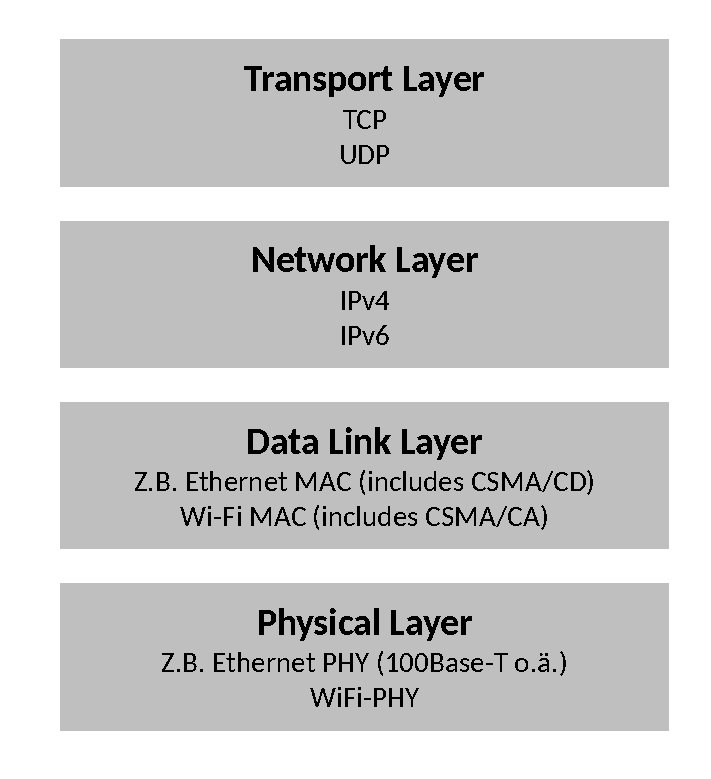
\includegraphics[width=\textwidth/2]{Grafiken-Alex/internet-osi.pdf}
	\caption{Beispielhafter Aufbau der ersten vier Schichten des OSI-Modells eines internetfähigen Geräts}
	\label{internet-osi}
\end{figure}
\begin{itemize}
	\item Layer 1 und 2 des OSI-Modells werden für gewöhnlich durch Techniken nach IEEE802.11 (Wi-Fi) oder IEEE802.3 (Ethernet) realisiert. Diese Normen sind nicht zwingend notwendig, um als Teilnehmer im Internet aufzutreten, sind aber gängige Lösungen.
	\item Zentraler Bestandteil des Internets ist das Internet Protocol (IP) auf Layer 3. Erst durch dessen Implementierung kann ein Gerät am Internet teilnehmen.
	\item Auf Layer 4 sind die Protokolle UDP (User Datagram Protocol) und TCP (Transmission Control Protocol) gängig, um verbindungslos (UDP) oder verbindungsorientiert (TCP) Daten zu verschicken.
\end{itemize}
Somit ergibt sich ein Aufbau der ersten vier Schichten des OSI-Modells wie in Grafik \ref{internet-osi}. 

Will man nun - wie es im Internet der Dinge häufig der Fall ist - von einem Sensor Daten zur Verwaltung an einen zentralen Server schicken, so ist der Einsatz von UDP sinnvoll. Es handelt sich ohnehin meist um kleine Datensätze, die die Größe eines einzelnen IP-Pakets nicht selten nicht überschreiten. Ein komplexer Verbindungsaufbau wie bei TCP ist hierzu nicht nötig. Ein unterwegs verloren gegangenes Paket richtet durch die ständige Aktualisierung von Sensordaten kaum großen Schaden an.\\
Auf Layer 3 ist der Einsatz von IP obligatorisch. Weil es sich bei IPv4 um ein veraltetes Protokoll handelt, das immer mehr von IPv6 verdrängt und moderne, zukunftsfähige Sensornetzwerke kaum noch darauf setzen, wird in dieser Ausarbeitung nur IPv6 betrachtet.\\
Bei den beiden unteren Layern ist der Einsatz kabelgebundener Lösungen kaum realistisch. Sensoren sollen die Möglichkeit bieten, ohne großen Montageaufwand flexibel eingesetzt werden zu können. Durch den geringen Stromverbrauch reichen schon einfache Knopfzellenbatterien als Energielieferant, weshalb eine Verlegung von Kabeln nur zu Kommunikationszwecken nicht sinnvoll wäre. Lösungen wie Ethernet fallen somit weg und auf den ersten Blick erscheint der Einsatz von Wi-Fi sinnvoll. Somit ergäbe sich ein tatsächlicher Aufbau der ersten vier Schichten des OSI-Modells wie in Grafik \ref{sensor-osi} gezeigt.
\begin{figure}
	\centering
	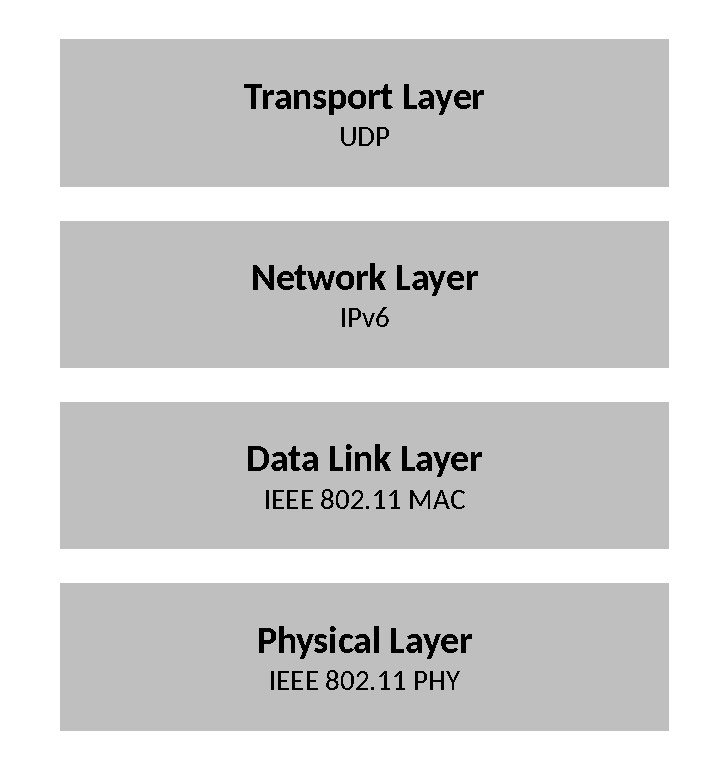
\includegraphics[width=\textwidth/2]{Grafiken-Alex/sensor-osi.pdf}
	\caption{Theoretisch möglicher Aufbau der ersten vier Schichten des OSI-Modells für einen Sensor}
	\label{sensor-osi}
\end{figure}
Herkömmliche Funkprotokolle - IEEE 802.11 alias Wi-Fi sei hier nur exemplarisch - bedienen die Anforderungen moderner Applikationen. Diese Anforderungen lassen sich zum größten Teil in einem Wort zusammenfassen: Datendurchsatz. Heutige Applikationen für Endanwender benötigen nicht selten einen Datendurchsatz im Bereich vieler Mbit/s. Diese Datenraten werden durch eine hohe Leistungsaufnahme entsprechender Module erkauft. So kann die Leistungsaufnahme eines einfachen Wi-Fi-fähigen SoC (System on a Chip) wie des ESP8266EX der Firma Espressif Systems durchaus 500mW erreichen \cite{esp8266}. Das ist unter Betracht der Tatsache, dass Knopfzellenbatterien für gewöhnlich nicht mehr als 3000mWh Energie speichern ein viel zu hoher Wert. \\
Sensor-Netzwerken benötigen im Gegensatz dazu nur geringe Datenraten, da nur wenige Daten - durchaus im Bereich einiger Bytes - verschickt werden. Andererseits ist hier ganz besonders auf die Leistungsaufnahme zu achten. Um diesen außergewöhnlichen Anforderungen gerecht zu werden, wurde eine Funktechnologie entwickelt und in IEEE 802.15.4 genormt. Weil man bei dieser Technologie auf einen einheitlichen Namen verzichtete - sie wird meist einfach als IEEE 802.15.4 bezeichnet - wird sie in dieser Ausarbeitung 15.4 genannt. \\
Der Standard 15.4 definiert Physical- und Mac-Layer eines Übertragungsprotokolls für Wireless Personal Area Networks (WPAN). Durch lange Ruhephasen wird hier die Leistungsaufnahme einzelner Netzteilnehmer so weit reduziert, dass die gängigen Akkulaufzeiten sich für gewöhnlich im Bereich vieler Monate bewegen. Der Preis dafür ist eine geringe Datenrate von maximal 250 kBit/s bzw. im Sub-1-GHz-Netz sogar nur 40 kBit/s. Was bei anderen Anwendungen absolut inakzeptabel wäre, reicht aber in diesem Falls absolut aus, um einfach Sensordaten ausreichend schnell zu übermitteln. \\
Eine Eigenschaft von 15.4 ist die maximale Paketgröße von 127 Bytes. IPv6 fordert jedoch eine Maximum Transmission Unit (MTU) von 1280 Byte. Das bedeutet, dass IPv6 vom auf Layer 2 eingesetzten Protokoll fordert, ein Paket mit maximal 1280 Bytes zu übertragen. Damit ist 15.4 als Übertragungsprotokoll eine IP-Pakets zunächst gar nicht möglich. Darüber hinaus hat der Header des IPv6-Protokolls eine Größe von 40 Bytes. Gemeinsam mit dem 8 Byte großen UDP-Header und dem 25 Byte großen MAC-Header von 15.4 blieben in einem Paket gerade mal 54 Byte für die Payload, wodurch sich die Datenrate von Nutzdaten auf ca. 17 kBit/s im Sub-1-GHz-Netz reduziert.\cite{grundlagen6lowpan} \\
Diese beiden Hindernisse verlangen von einer Implementierung von IPv6 auf Basis von 15.4 zwei Eigenschaften:
\begin{itemize}
	\item Fragmentierungs- und Defragmentierungsebene für IP-Pakete einführen, um die MTU nicht zu verletzen.
	\item Header von IP und UDP möglichst weit komprimieren, um den Anteil an Nutzdaten in einem Datenpaket zu erhöhen.
\end{itemize}
\begin{figure}
	\centering
	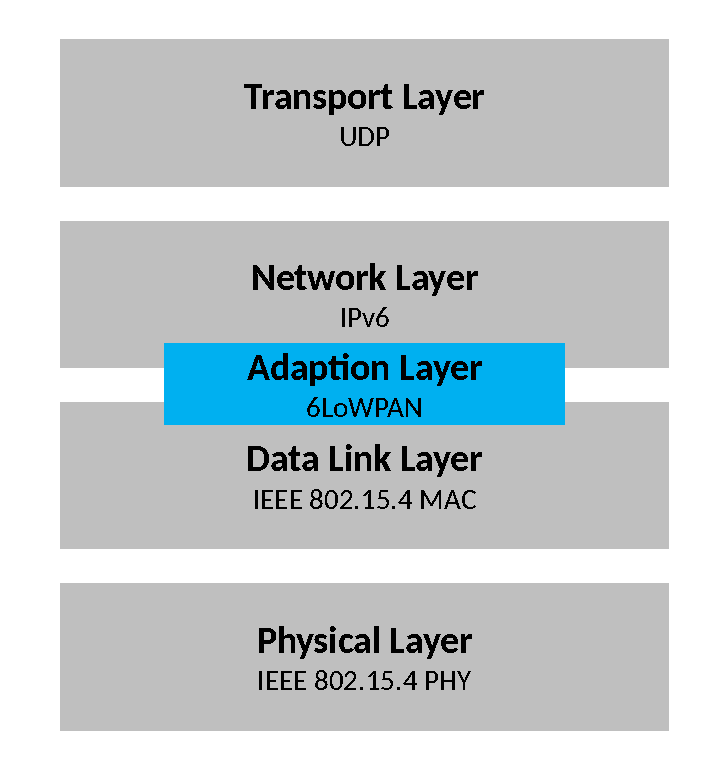
\includegraphics[width=\textwidth/2]{Grafiken-Alex/6lowpan-osi.pdf}
	\caption{Aufbau der ersten vier Schichten des OSI-Modells unter Verwendung von 6LoWPAN}
	\label{6lowpan-osi}
\end{figure}
Um beiden Anforderungen gerecht zu werden, wurde die 6LoWPAN Zwischenschicht eingeführt. Diese gliedert sich zwischen Layer 2 (15.4 MAC) und Layer 3 (IPv6) als Adaptionslayer ein und ermöglicht so die Nutzung von IP und darauf aufbauend UDP auf Basis von 15.4. Darüber hinaus muss zur Kommunikation nach außen mindestens ein Netzwerkteilnehmer in der Lage sein, Datenpakete, die mit 6LoWPAN verschickt wurden in ganz normale UDP/IP-Pakete zu wandeln und über eine herkömmliche Übertragungstechnologie weiterzuleiten. Erst dadurch wird ein einzelner Sensor fähig, am Internet teilzunehmen. Die ersten vier Schichten des OSI-Modells eines solchen Sensors ergeben sich dann also wie in Graphik \ref{6lowpan-osi} gezeigt.
  
 
